\documentclass[12pt, twoside]{article}
\usepackage[francais]{babel}
\usepackage[T1]{fontenc}
\usepackage[latin1]{inputenc}
\usepackage[left=6mm, right=6mm, top=3mm, bottom=3mm]{geometry}
\usepackage{float}
\usepackage{graphicx}
\usepackage{array}
\usepackage{multirow}
\usepackage{amsmath,amssymb,mathrsfs}
\usepackage{soul}
\usepackage{textcomp}
\usepackage{eurosym}
 \usepackage{variations}
\usepackage{tabvar}


\pagestyle{empty}

\begin{document}


\section*{\center{Devoir maison 4}}

\textit{Devoir � rendre sur feuille grand format petits
carreaux pour le \ul{mardi 1 f�vrier 2011}.}

\enskip


\textit{Remarque: La r�daction et la justifcation des r�sultats seront pris en
compte.}

\subsection*{Exercice 1}




\begin{tabular}{cc}
\begin{minipage}{13cm}

$\mathcal{L}$ est un cercle de centre E.
\begin{enumerate}
  \item Montrer que le triangle AFD est rectangle en F.
  \item Que peut-on dire des droites (CA) et (CB)? Justifier.
\end{enumerate}

\end{minipage}
&
\begin{minipage}{5cm}
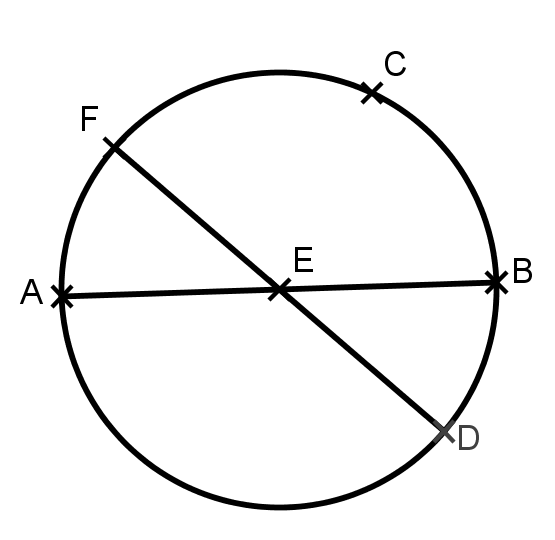
\includegraphics[width=40mm]{images/ex1.png}
\end{minipage}
\end{tabular}

 


\subsection*{Exercice 2}


A partir des informations port�es sur la figure suivante, d�terminer  les
longueurs MN et BD (la r�ponse devra �tre r�dig�e).

\begin{center}
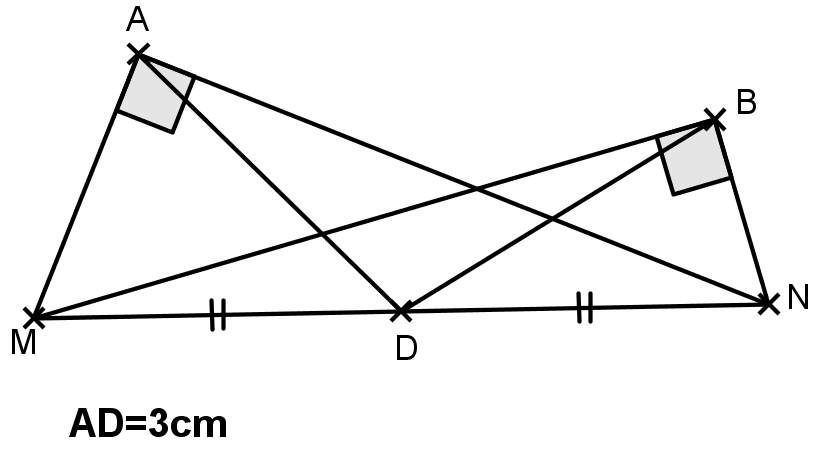
\includegraphics[width=55mm]{images/ex2.png} 
\end{center}


\subsection*{Exercice 3}

\begin{enumerate}
  \item Construire un triangle TOC tel que TO=8cm, $\widehat{TOC}=34$� et
  $\widehat{CTO}=56$�.
  \item D�montrer que le cercle de diam�tre [TO] passe par le point C.
\end{enumerate}


\subsection*{Exercice 4}

\begin{tabular}{cr}
\begin{minipage}{11cm}

Construire un point P tels que les triangles ABP et CDP soient rectangles en P.
Justifier votre r�ponse.

\enskip

(\textit{La construction se fera sur la photocopie et les explications seront
not�es sur votre feuille.})


\end{minipage}
&
\begin{minipage}{7cm}
\begin{center}
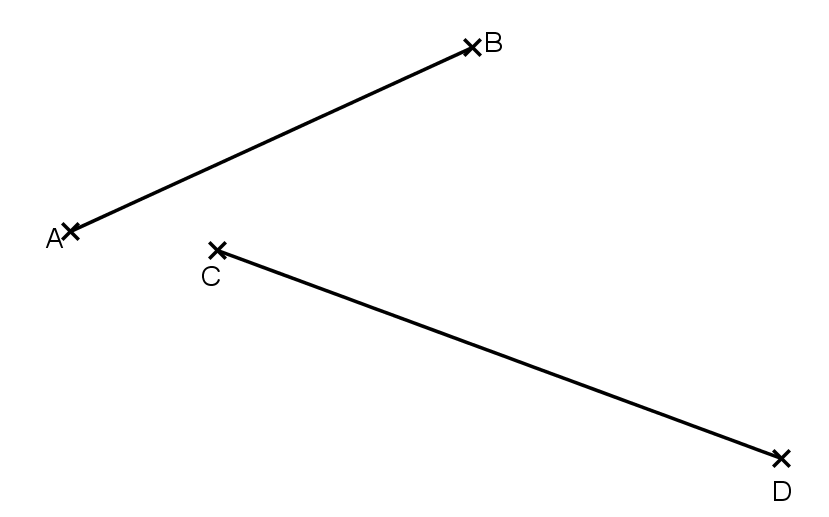
\includegraphics[width=65mm]{images/ex4.png}
\end{center}
\end{minipage} 
\end{tabular}


\subsection*{Exercice 5}

Sur un parcours sportif, un athl�te r�alise un temps de 45 minutes sur les 9
kilom�tres de la partie A puis met 1h30min pour les 15 kilom�tres de la partie
B.

\begin{enumerate}
  \item Calculer sa vitesse sur la partie A.
  \item Calculer sa vitesse sur la partie B.
  \item Calculer sa vitesse sur l'ensemble du parcours (arrondir les r�sultats
  au centi�me).
  \item Convertir les r�sultats des 3 premi�res questions en m/s (arrondir les
  r�sulats au centi�me).
\end{enumerate}
\end{document}
